In this section, we present the final results for each individual verilog 
filed we have submitted to the Tiny Tapeout initiative. The following figures 
Show our verilog designs in a phisical layout, and the Table\ \ref{tab:PorcentUtil} show 
a Porcentage utilize in length of waver per circuit.



\subsection{Multy stage path for delay measurements}

The multy stage path was submitted with no errors, and the final layout is shown in figure\ \ref{fig:delay_Layout}. The layout was designed to be as compact as possible, and the final area was 0.63\% (as showed in Table\ \ref*{tab:PorcentUtil}) of the total area of the chip. 

\begin{figure}[H]
    \centering
    \begin{subfigure}[b]{0.45\textwidth}
        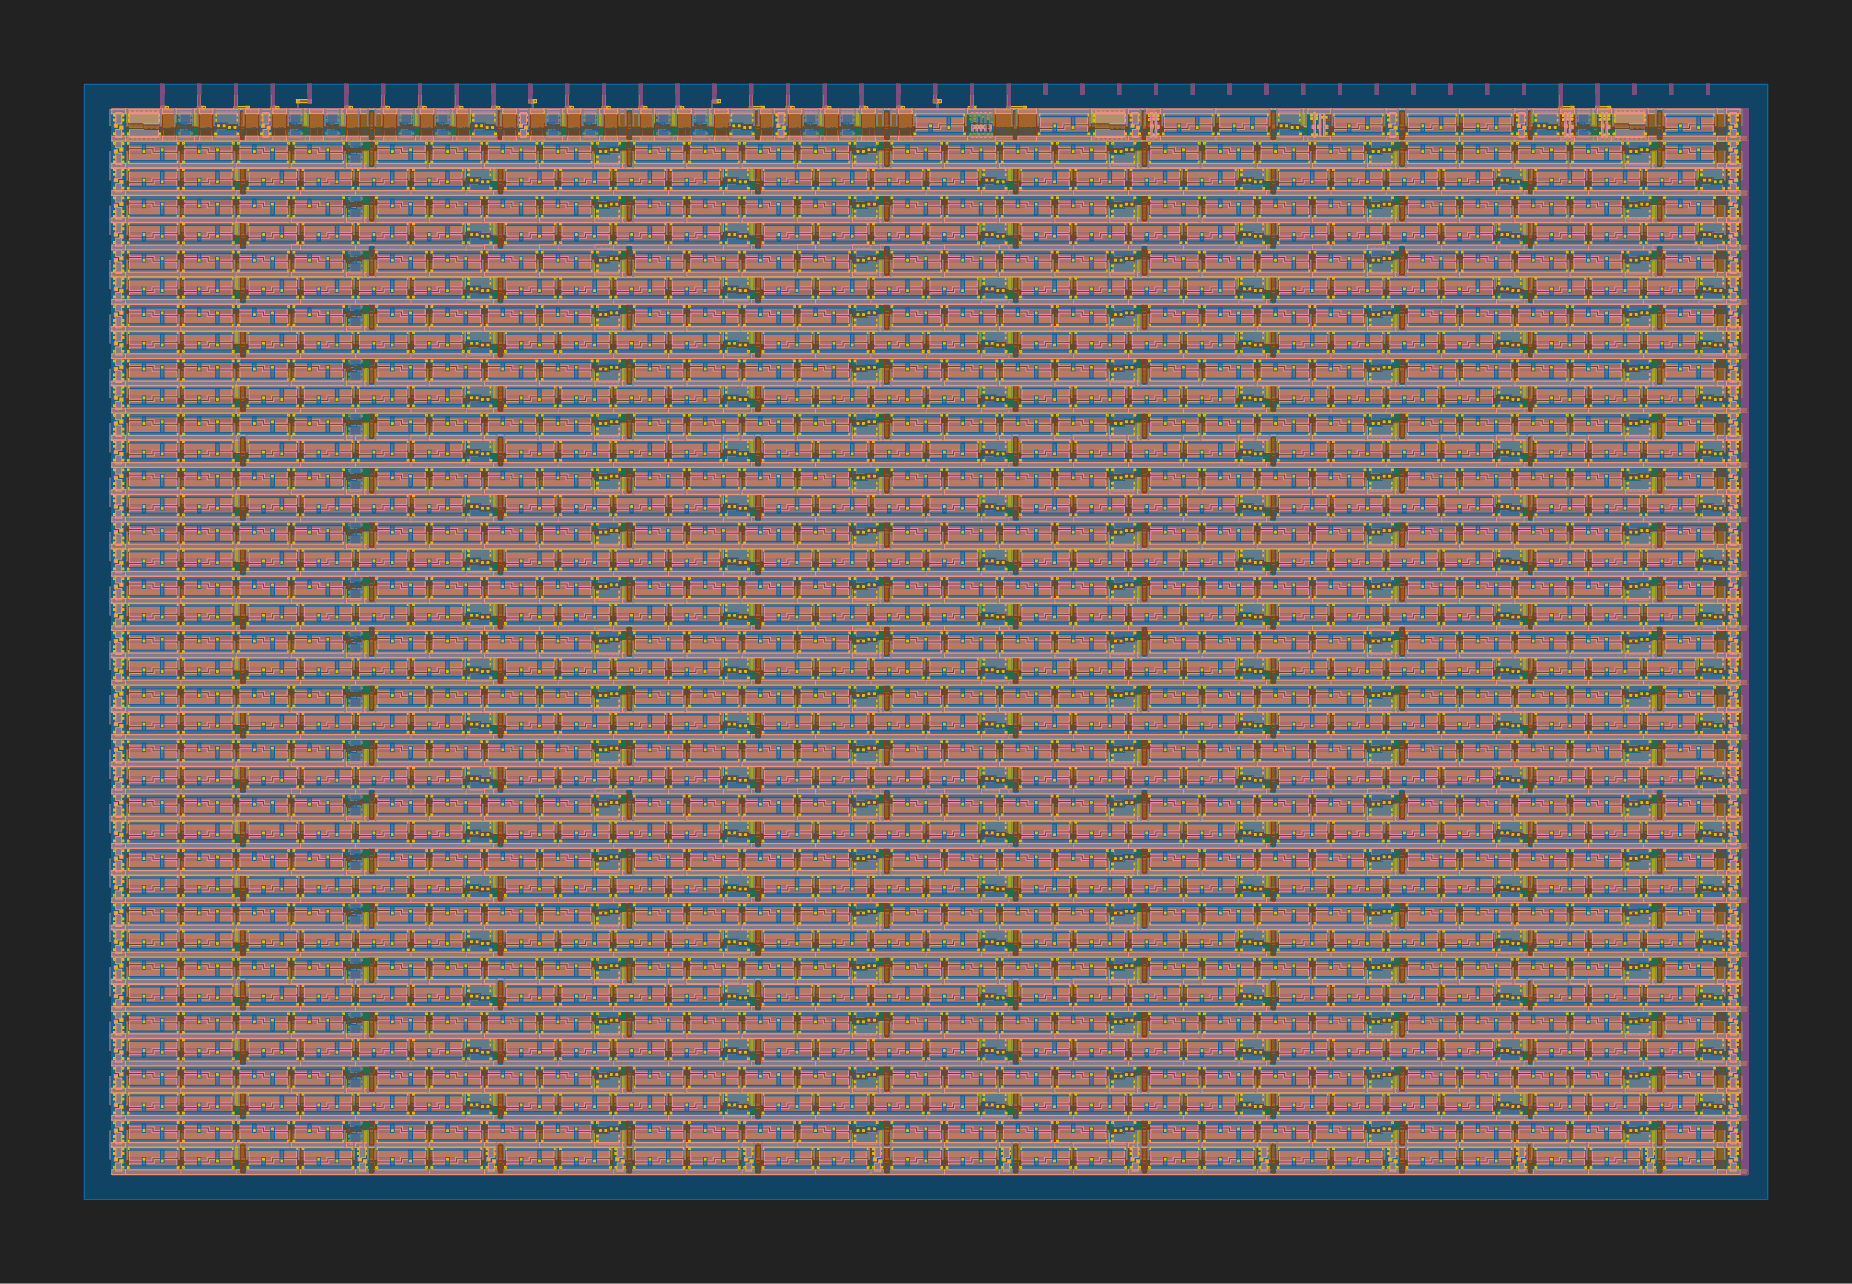
\includegraphics[width=\linewidth]{Pictures/Result_Delay_2D_View.png}
        \caption{View 2D}\label{fig:delay_2D}
    \end{subfigure}
    \begin{subfigure}[b]{0.45\textwidth}
        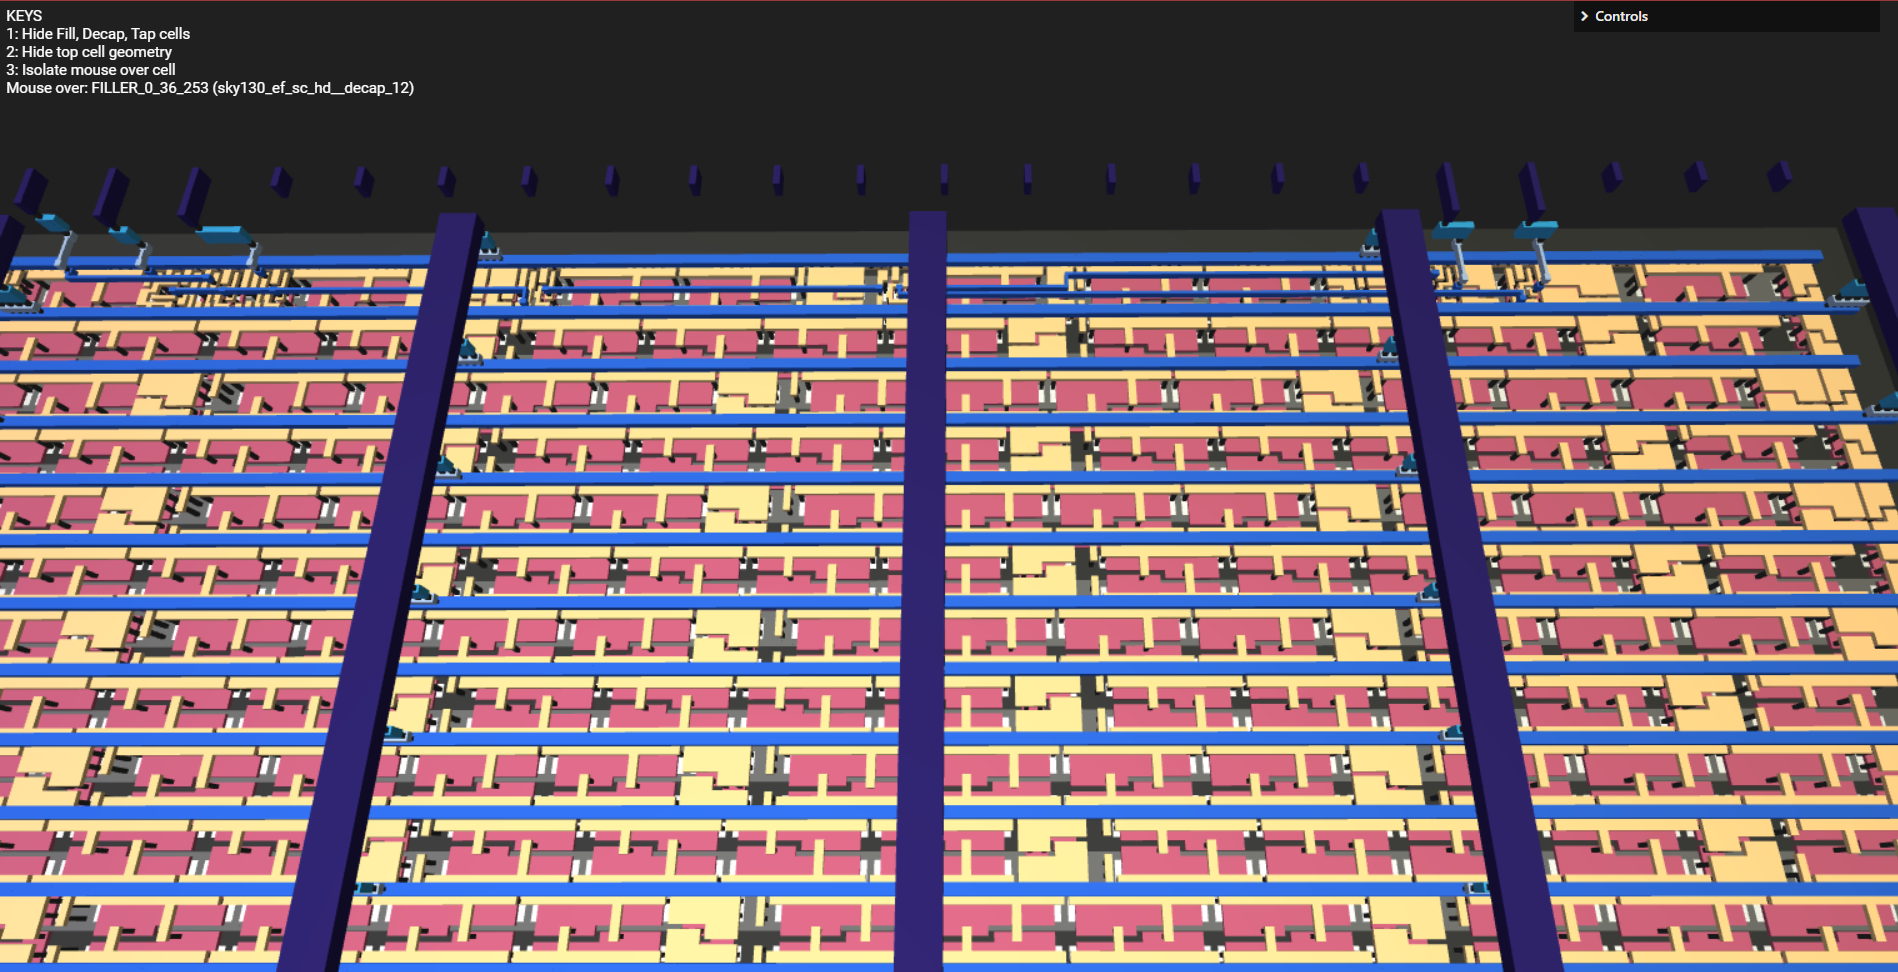
\includegraphics[width=\linewidth]{Pictures/Result_Delay_3D_View.png}
        \caption{View 3D}\label{fig:delay_3D}
    \end{subfigure}
    \caption{multy stage path for delay measurements layout}\label{fig:delay_Layout}
\end{figure}

\subsection{ASCII Text Printer Circuit}

The circuit ASCII text printer was submitted with no errors, and the final layout is shown in figure\ \ref{fig:ASCII_Layout}. The layout was designed to be as compact as possible, and the final area was 17.87\% (as showed in Table\ \ref*{tab:PorcentUtil}) of the total area of the chip.

\begin{figure}[H]
    \centering
    \begin{subfigure}[b]{0.45\textwidth}
        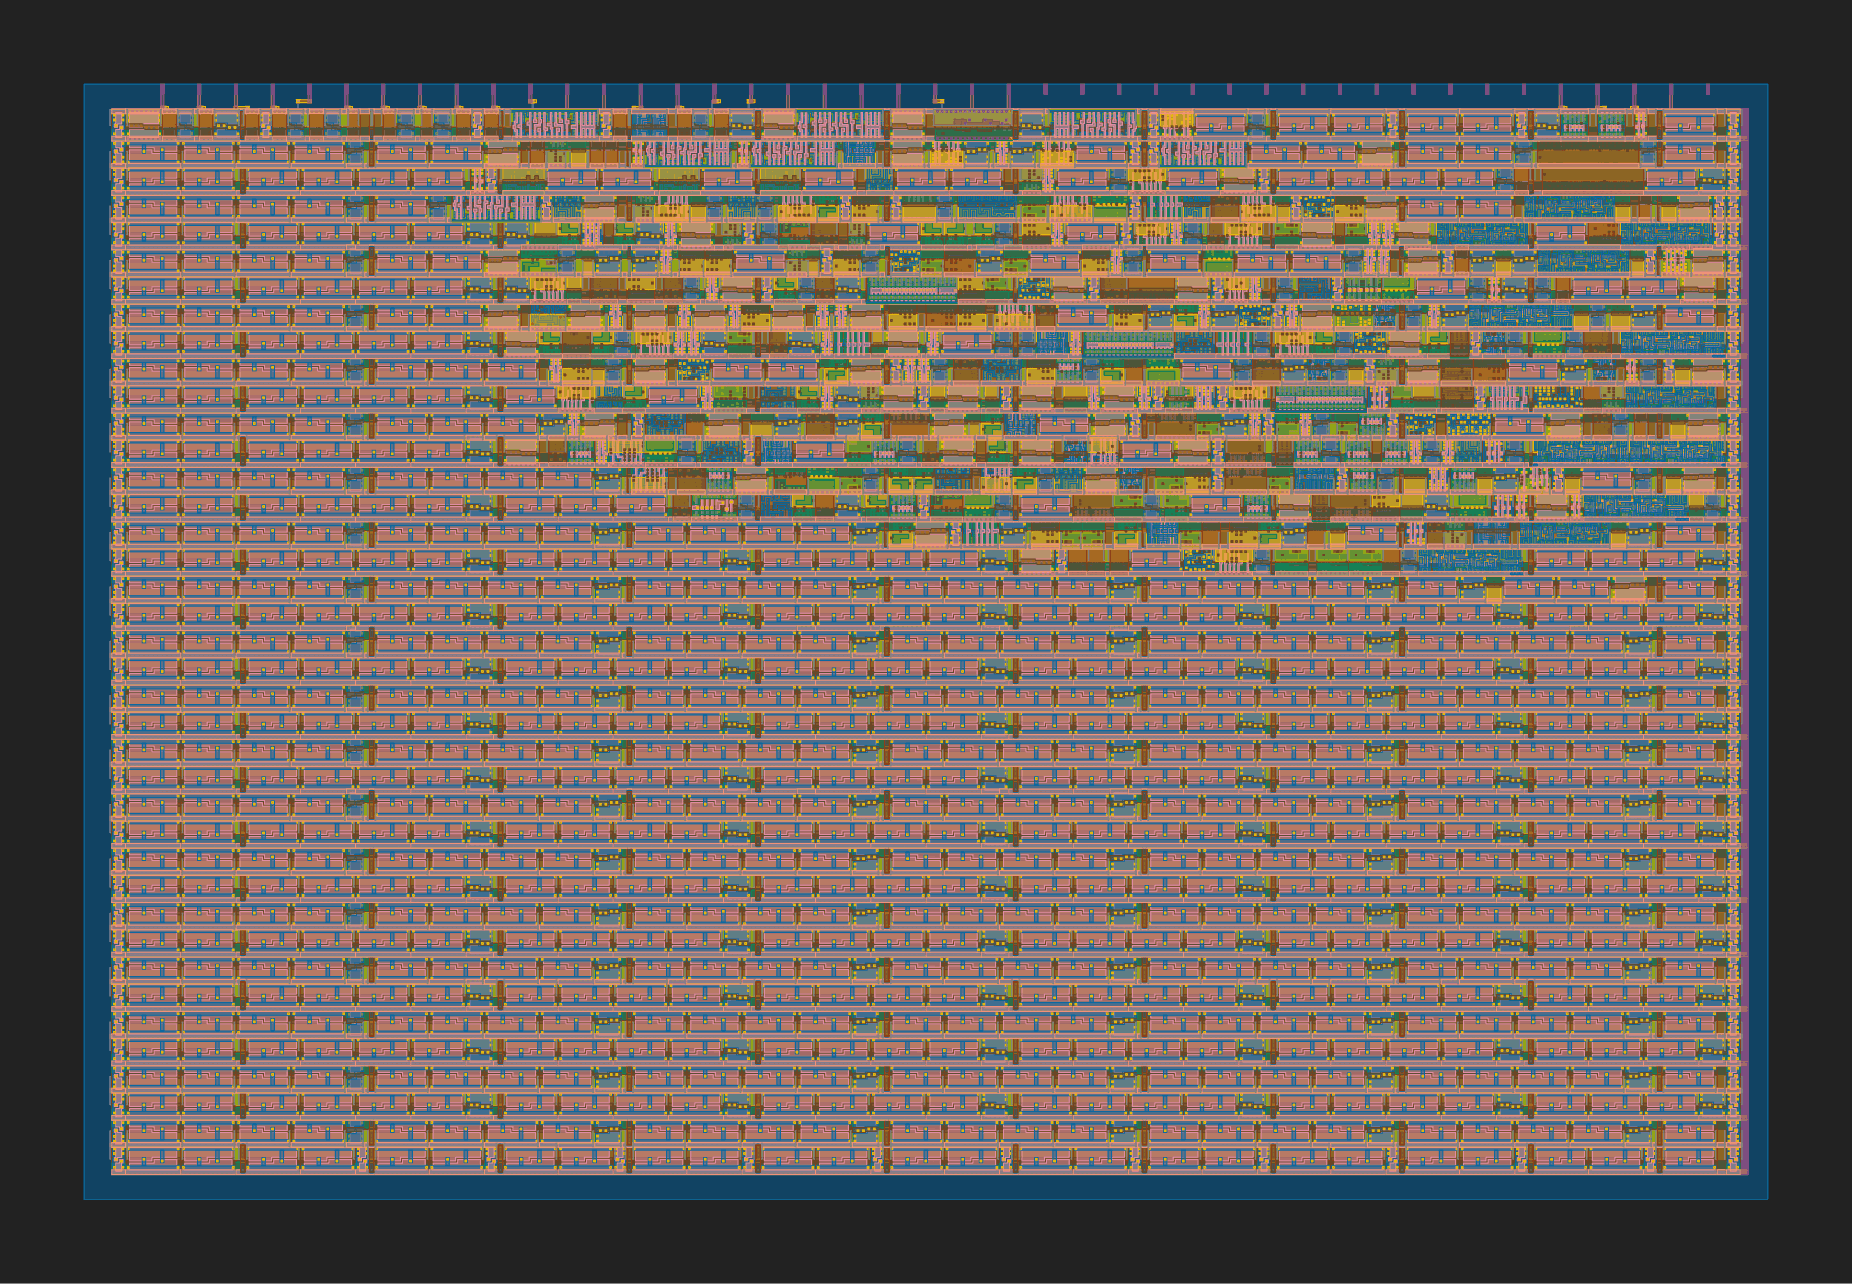
\includegraphics[width=\linewidth]{Pictures/Result_ASCII_2D_View.png}
        \caption{View 2D}\label{fig:ASCII_2D}
    \end{subfigure}
    \begin{subfigure}[b]{0.45\textwidth}
        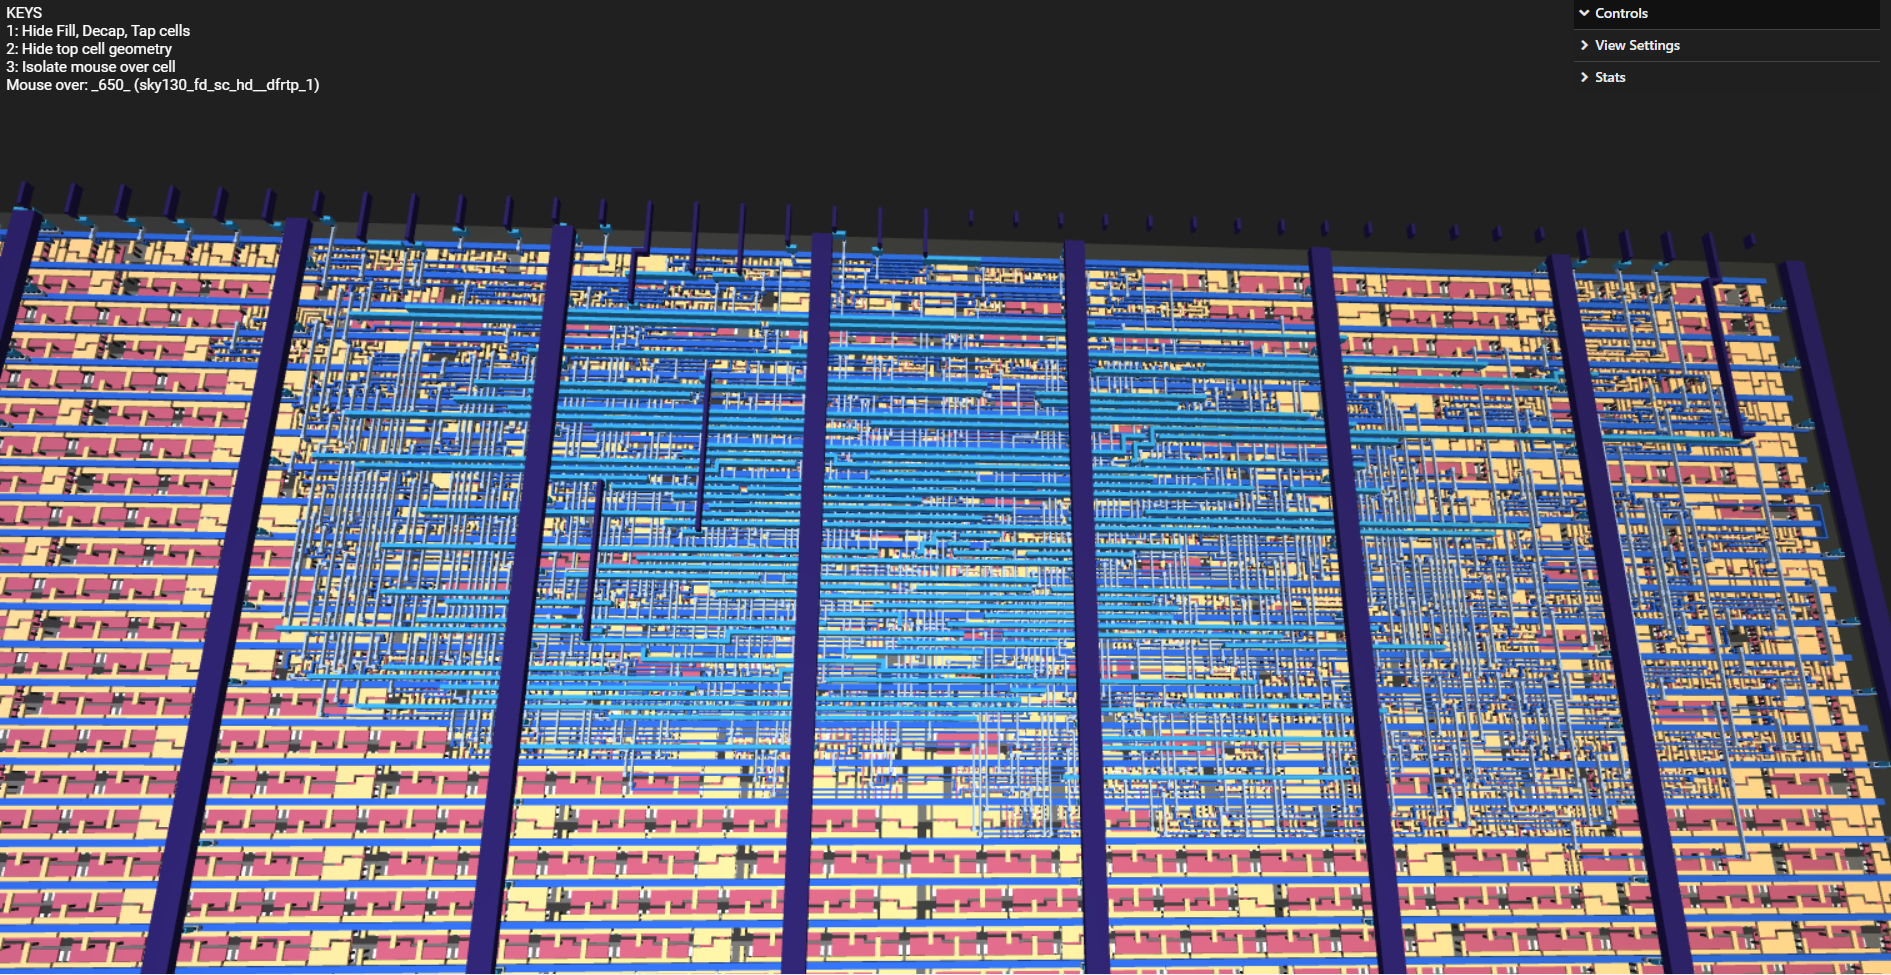
\includegraphics[width=\linewidth]{Pictures/Result_ASCII_3D_View.png}
        \caption{View 3D}\label{fig:ASCII_3D}
    \end{subfigure}
    \caption{ASCII text printer circuit layout}\label{fig:ASCII_Layout}
\end{figure}

\subsection{Implementation of the Pong game}

The circuit of the Pong game was submitted with no errors, and the final layout is shown in figure\ \ref{fig:Pong_Layout}. The layout was designed to be as compact as possible, and the final area was 28.82\% (as showed in Table\ \ref*{tab:PorcentUtil}) of the total area of the chip.

\begin{figure}[H]
    \centering
    \begin{subfigure}[b]{0.45\textwidth}
        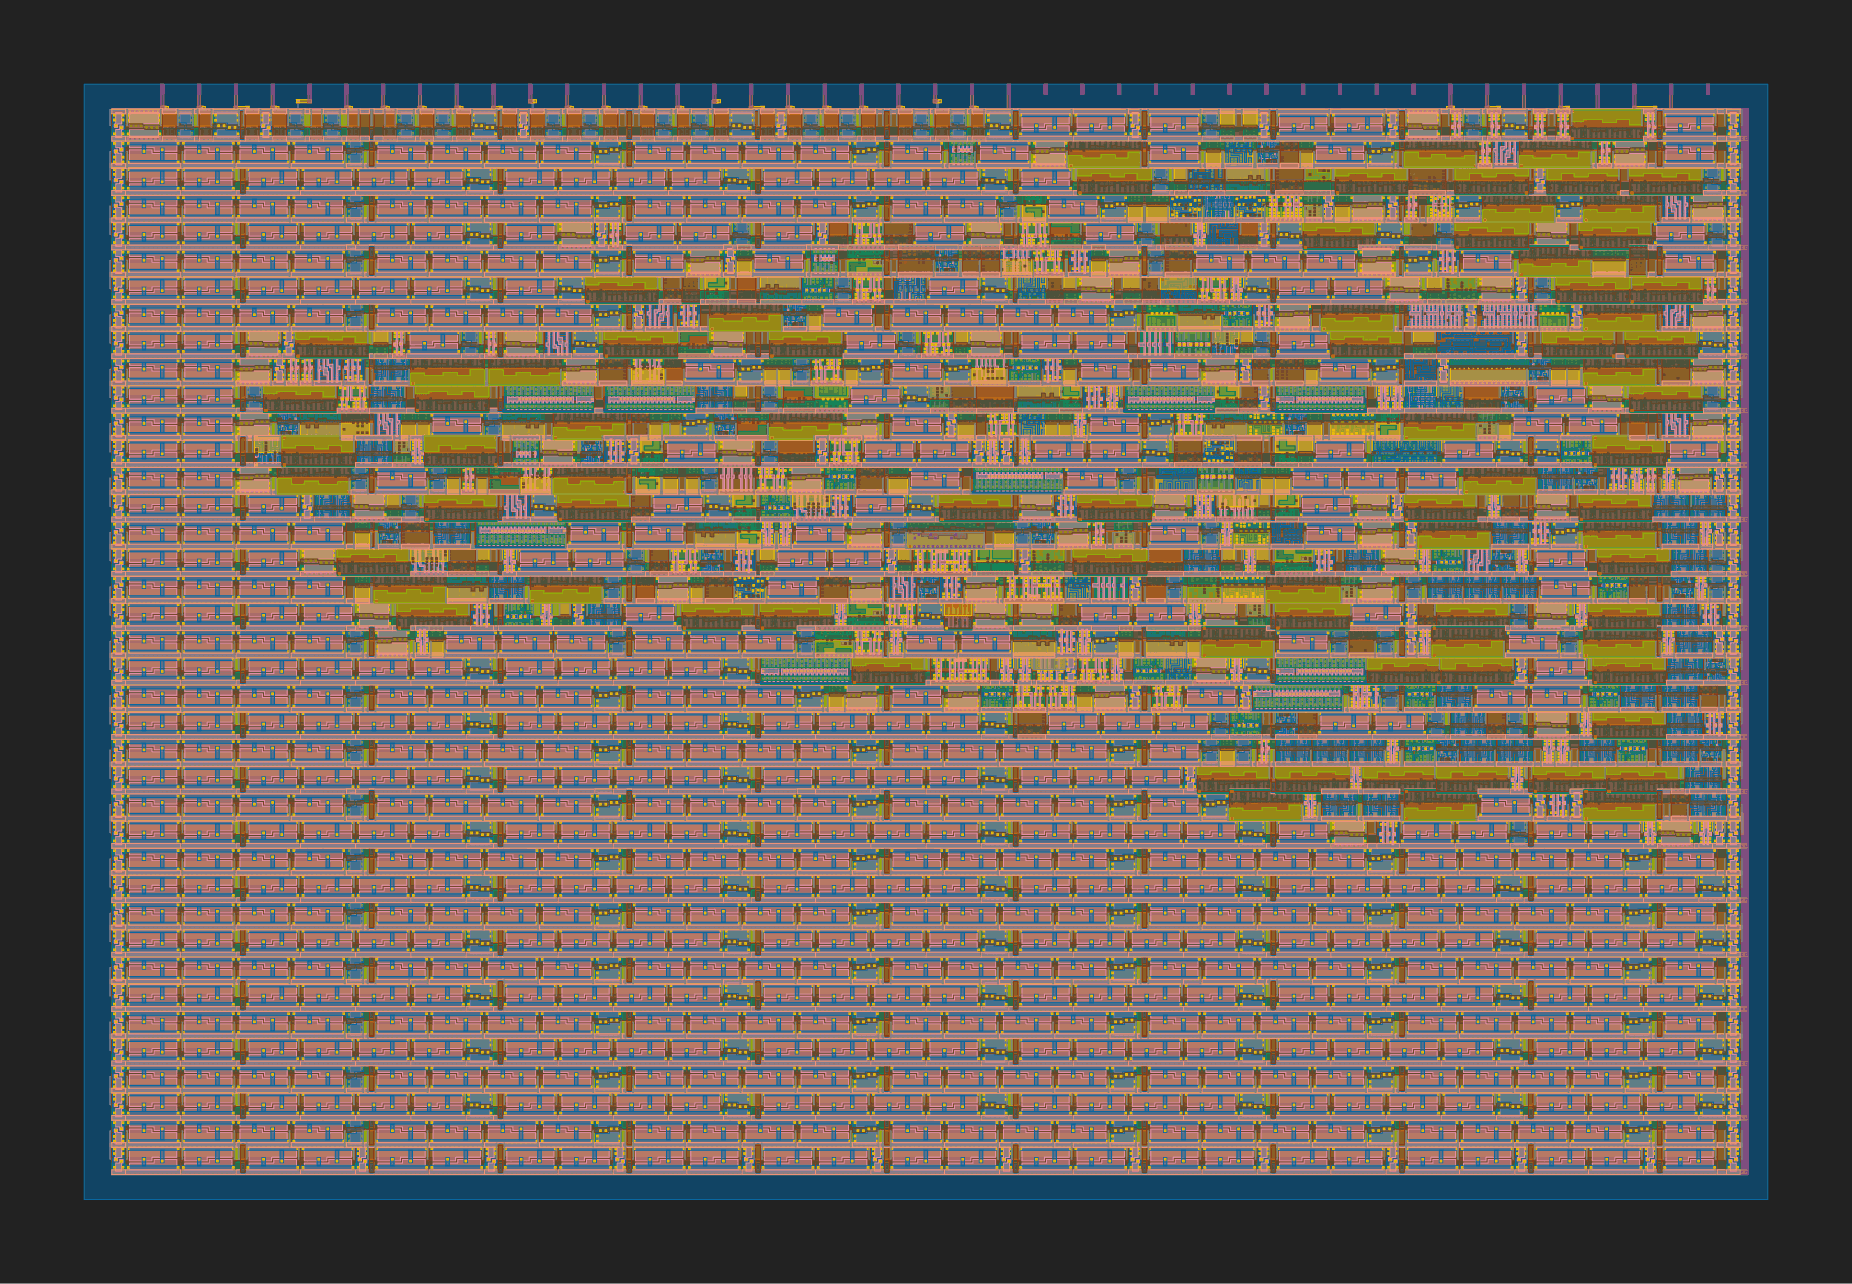
\includegraphics[width=\linewidth]{Pictures/Result_Pong_2D_View.png}
        \caption{View 2D}\label{fig:pong_2D}
    \end{subfigure}
    \begin{subfigure}[b]{0.45\textwidth}
        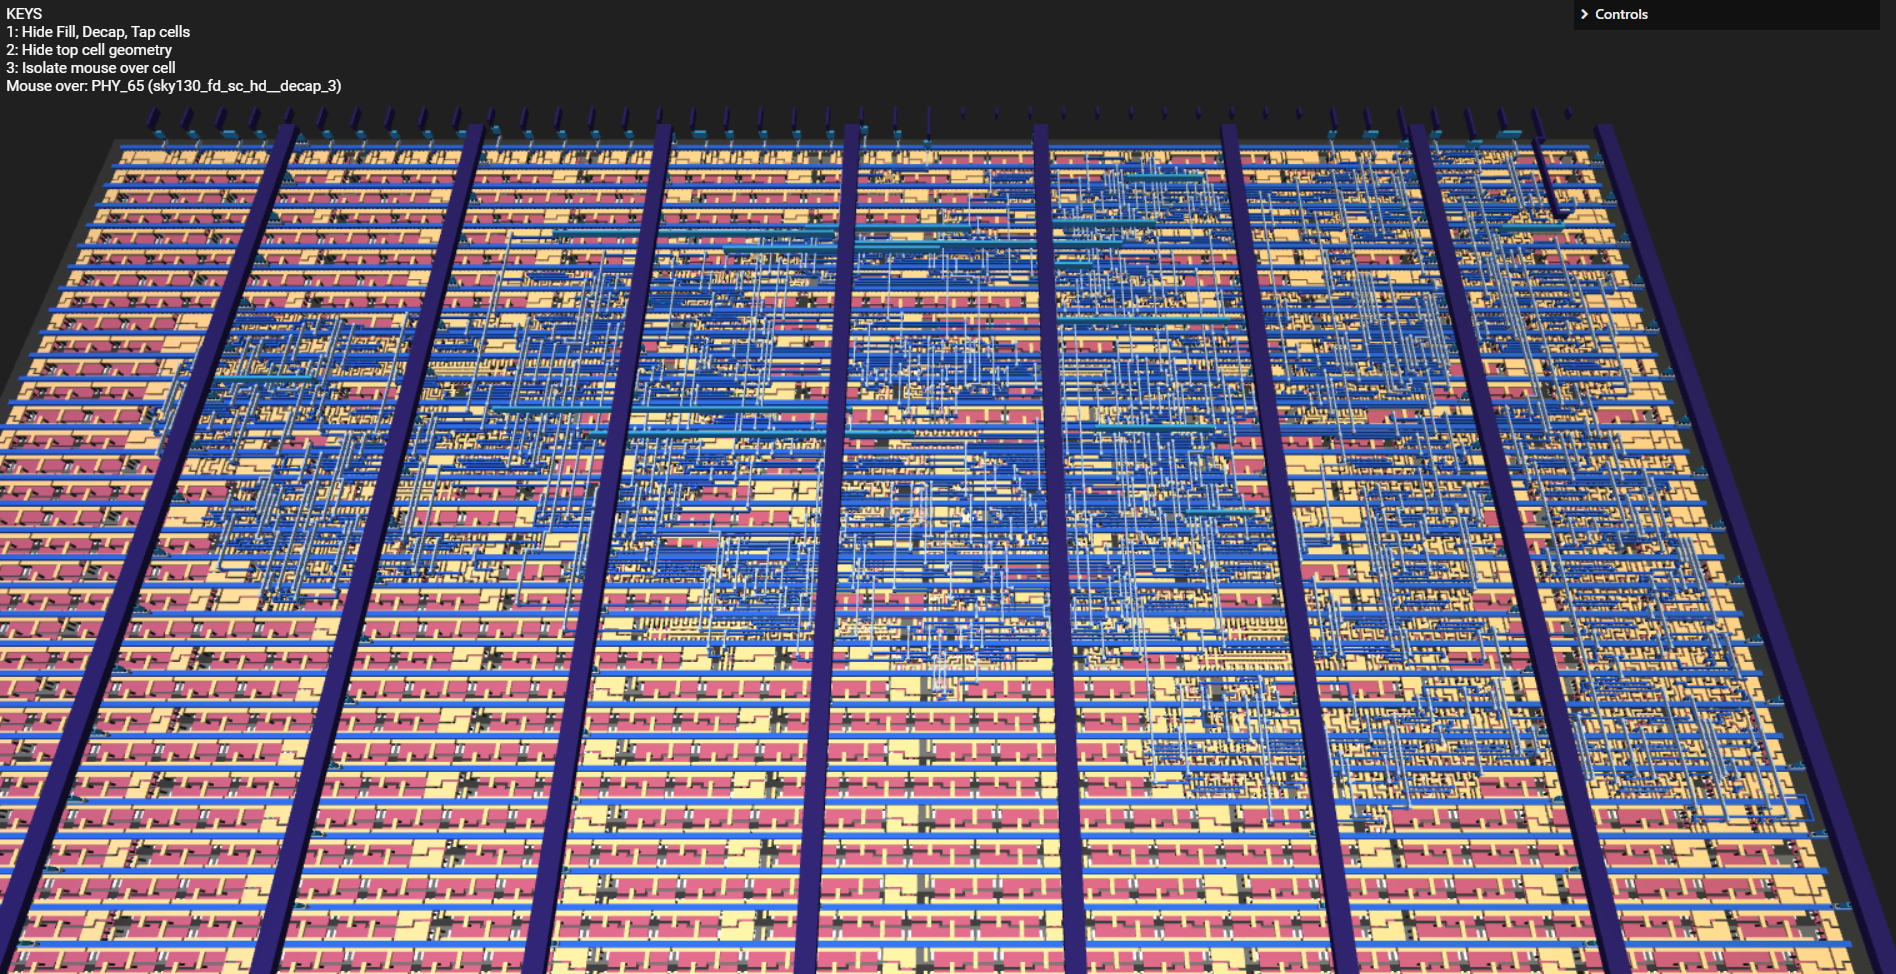
\includegraphics[width=\linewidth]{Pictures/Result_Pong_3D_View.png}
        \caption{View 3D}\label{fig:pong_3D}
    \end{subfigure}
    \caption{The Pong game layout}\label{fig:Pong_Layout}
\end{figure}

\subsection{Pulse Width Modulation Generator}

The circuit of the Pulse Width Modulation generator was submitted with no errors, and the final layout is shown in figure\ \ref{fig:PWM}. The layout was designed to be as compact as possible, and the final area was 9.59\% (as showed in Table\ \ref*{tab:PorcentUtil}) of the total area of the chip.

\begin{figure}[H]
    \centering
    \begin{subfigure}[b]{0.45\textwidth}
        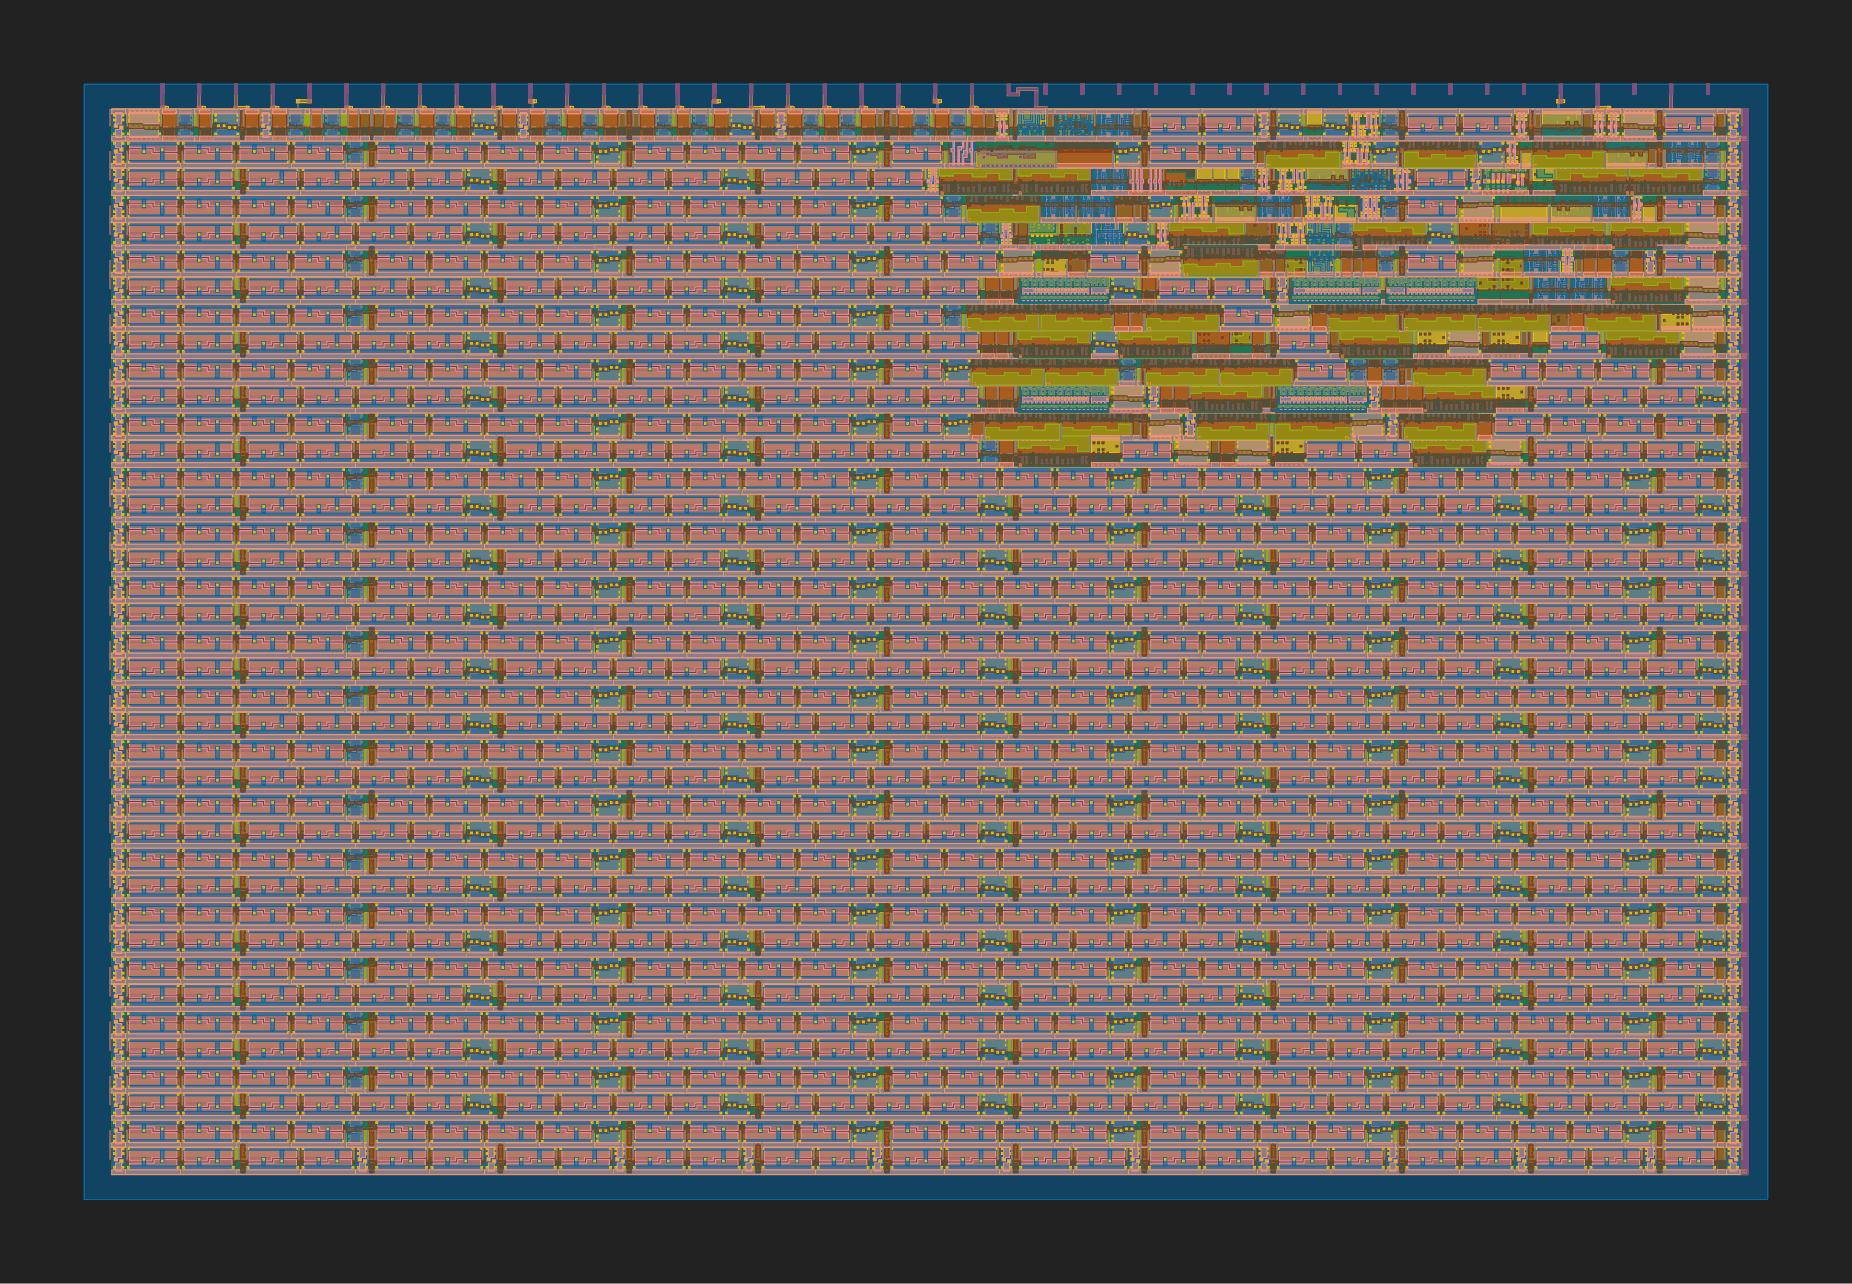
\includegraphics[width=\linewidth]{Pictures/Result_PWM_2D_View.png}
        \caption{View 2D}\label{fig:PWM_2D}
    \end{subfigure}
    \begin{subfigure}[b]{0.45\textwidth}
        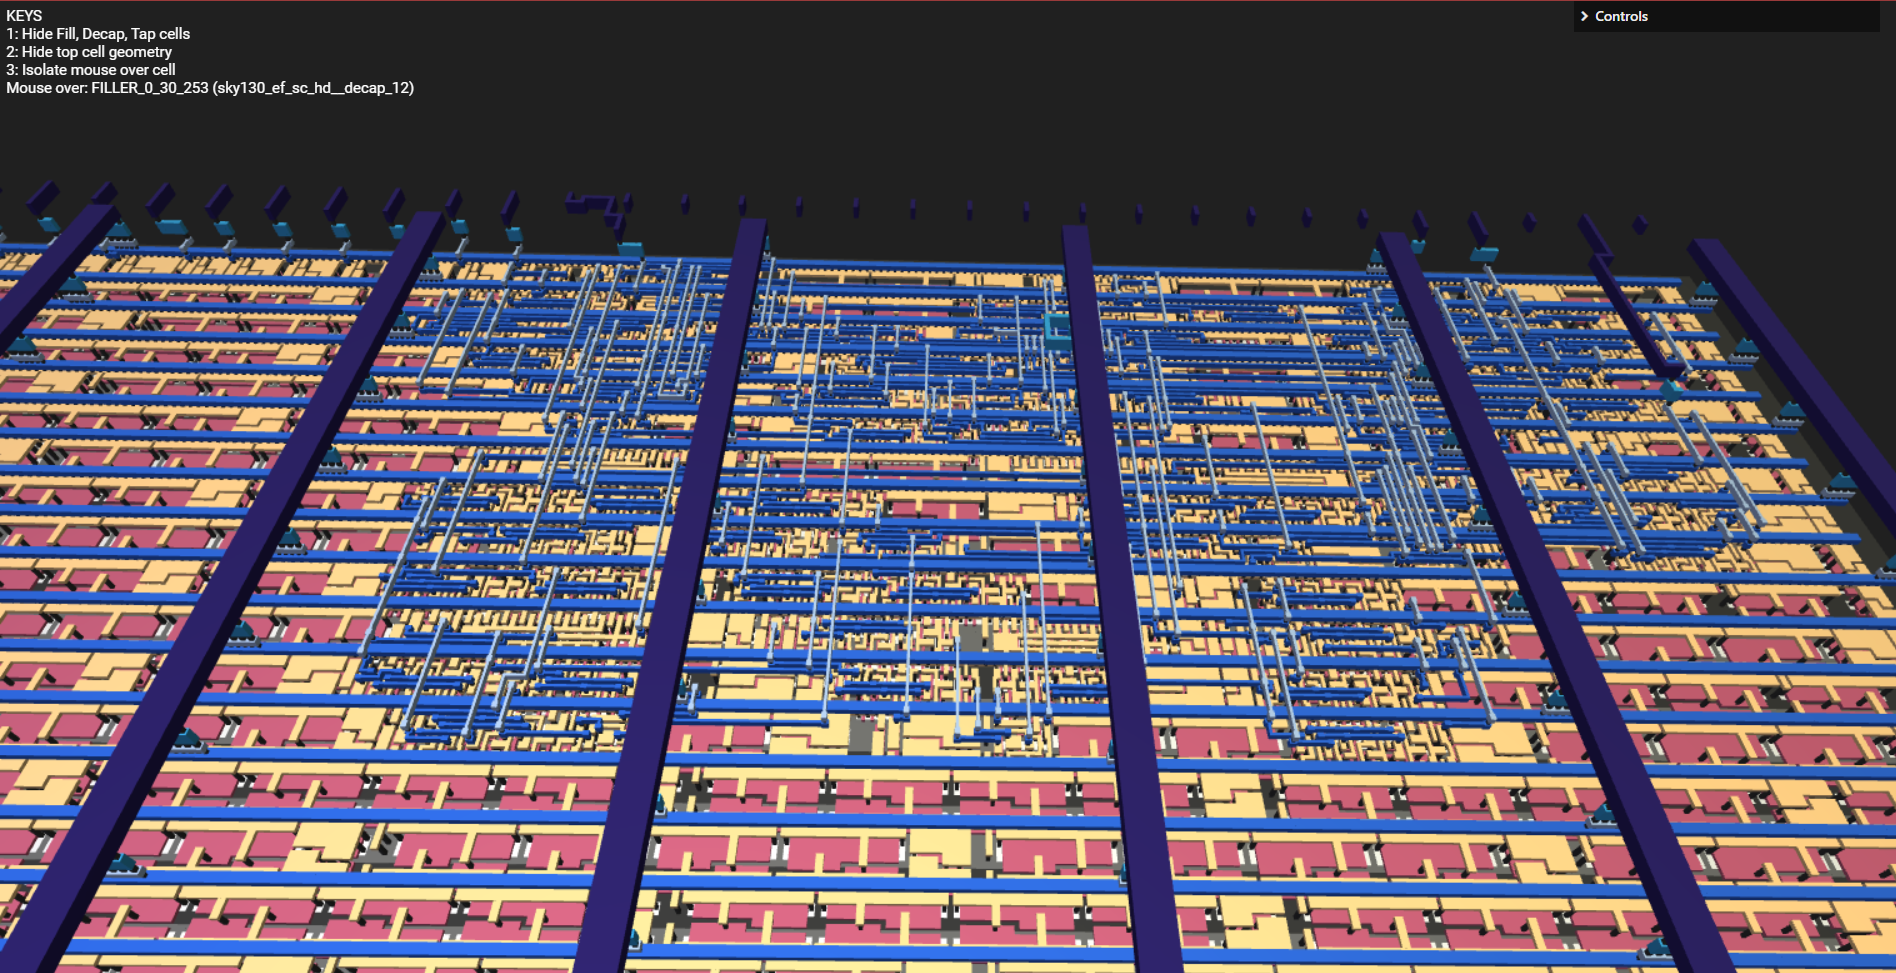
\includegraphics[width=\linewidth]{Pictures/Result_PWM_3D_View.png}
        \caption{View 3D}\label{fig:PWM_3D}
    \end{subfigure}
    \caption{Pulse Width Modulation generator layout}\label{fig:PWM}
\end{figure}

% Please add the following required packages to your document preamble:
% \usepackage{graphicx}
\begin{table}[H]
    \centering
    \resizebox{\columnwidth}{!}{%
    \begin{tabular}{cc}
    \hline
    Circuit                                 & Porcentage utilize(\%) \\ \hline
    Multy stage path for delay measurements & 0.63                  \\
    ASCII Text Printer Circuit              & 17.87                 \\
    Implementation of the Pong game         & 28.82                 \\
    Pulse Width Modulation Generator        & 9.59                  \\ \hline
    \end{tabular}%
    }
    \caption{Porcentaje utilize in length of waver per circuit}\label{tab:PorcentUtil}
    \end{table}
The links to the repositories with Verilog files are in the Appendix\ \ref{sec:GitHub}. In the repositories can find the Verilog files, the final layout, and the description of each circuit.